\documentclass[letterpaper,10pt]{memoir}


% === AUTOR === (((
\author{\textit{Por Erick I. Rodríguez Juárez.}}
% )))

% === PAQUETES === (((
% \usepackage{makeidx}
% \usepackage{xltxtra}
\usepackage{amsfonts}
\usepackage{amsmath}
\usepackage{amssymb}
% \usepackage{fullpage}
\usepackage{tikz}
\usetikzlibrary{arrows.meta}
\usepackage{graphicx}
% )))

% === TIPOGRAFÍA === (((
% \setmainfont[
  % BoldFont       = bodonibi,
	% ItalicFont     = Century modern italic2.ttf,
	% BoldItalicFont = bodonibi,
	% SmallCapsFont  = lmromancaps10-regular.otf
% ]{Century_modern.ttf}
% )))

% === COMANDOS === (((
% \newcommand{\dis}{\displaystyle}
% \newcommand{\qed}{\hspace{0.5cm}\rule{0.16cm}{0.4cm}}
% \newcommand{\operator}[1]{\mathop{\vphantom{\sum}\mathchoice
% {\vcenter{\hbox{\huge $#1$}}}
% {\vcenter{\hbox{\Large $#1$}}}{#1}{#1}}\displaylimits}
% \newcommand{\suma}{\operator{
\includegraphics[scale=0.09]{FOTOS/Sigma.png}}}
% \setlength{\parindent}{0mm}
% )))

% === ITALICA EN ENTORNO MATEMÁTICO === (((
% \DeclareSymbolFont{italics}{\encodingdefault}{\rmdefault}{m}{it}
% \DeclareSymbolFontAlphabet{\mathit}{italics}
% \ExplSyntaxOn
% \int_step_inline:nnnn { `A } { 1 } { `Z }
 % {  \exp_args:Nf \DeclareMathSymbol{\char_generate:nn{#1}{11}}{\mathalpha}{italics}{#1} }
% \int_step_inline:nnnn { `a } { 1 } { `z } {  \exp_args:Nf \DeclareMathSymbol{\char_generate:nn{#1}{11}}{\mathalpha}{italics}{#1}}
% \ExplSyntaxOff
% )))


\begin{document}

\titulo

\begin{enumerate}
	\item En los siguientes problemas se proporciona la solución uniparamétrica de las E.D. Encuentre la solución de los P.V.I. formados por la E.D. y la condición inicial que se proporciona. De el intervalo de definición más grande en el cual se define la solución y esboza la gráfica (si es necesario usa una Gogebra o WolframAlpha).
		\begin{enumerate}
			\item P.V.I. \(y \,' =y-y^3\) con \(y(0) =- \dfrac{1}{3}\). \textbf{Solución.} Sol. Gral. \(y(x) = \dfrac{1}{1+ce^{-x}}\).
			\item P.V.I. \(y \,' +2xy^2=0\) con \(y(-2) = \dfrac{1}{2}\). \textbf{Solución.} Sol. Gral. \(y(x) = \dfrac{1}{x^2+c}\).
		\end{enumerate}
	\item Sea \(y(x) =2x+ce^{-x}\) de la ecuación diferencial \(y \,' +y=2+2x\).
		\begin{enumerate}
			\item Determina la solución particular que pasa por el punto \((x_0,y_0)\).
			\item Considera el punto \((1,1)\) e indica que función solución pasa por dicho punto.
			\item Esboza la familia de soluciones de la E.D. dada e identifica la curva de la función solución encontrada en b).
		\end{enumerate}
	\item Resuelve el problema de valor inicial \(ty'+2y= \sin  t\), \(y(\pi /2)=1\), \(t>0\).  Utilice WolframAlpha para determinar la solución general de la ecuación diferencial.
	\item Compruebe que \(3x^2+y^2=c\) es la solución general implícita de la E.D. \(\dfrac{dy}{dx} =- \dfrac{3x}{y}\).
		\begin{enumerate}
			\item Encuentre la solución particular implícita que satisface el P.V.I conformado por la E.D. dada y la condición inicial \(y(-2) =3\).
			\item Encuentre las soluciones explícitas  de la E.D. \(y=y(x)\) e indica cual es su intervalo de definición.
			\item Grafíca algunas soluciones explícitas de la ecuación diferencial e indica cual gráfica corresponde a la solución del P.V.I.
		\end{enumerate}
	\item Aproveche que se da la solución general de las ecuaciones diferenciales, para determinar una solución de los problemas de valores iniciales formados por la ecuación y las condiciones iniciales indicadas. Esboza la gráfica de la solución de los P.V.I. para mostrar la interpretación geométrica de las condiciones iniciales.
		\begin{enumerate}
			\item \(x(t) =c_1 \cos t+c_2 \sin t\), \(x '' +x=0\).
				\begin{enumerate}
					\item \(x(0) =-1\), \(x \,' (0) =8\).
					\item \(x \Big(\dfrac \pi 6\Big) = \dfrac{1}{2}\), \(x \,' \Big(\dfrac{\pi}{6}\Big) =0\).
				\end{enumerate}
			\item \(y(x) =c_1e^x+c_2e^{3x} + \dfrac{1}{3}\), \(y '' -4y \,' +3y=1\).
				\begin{enumerate}
					\item \(y(0) =y \,' (0) =1\).
					\item \(y(-1) =0\), \(y \,' (-1) =-5\).
				\end{enumerate}
		\end{enumerate}
\end{enumerate}

{\large \textbf{Problemas para Discusión.}}
\begin{enumerate}
	\item Encuentra una función \(y=y(x)\) cuya gráfica en cada punto \((x,y)\) tiene la pendiente dada por \(8e^{2x} +6x\) y la ordenada al origen \((0,9)\).
	\item En la Figura muestra las gráficas de cuatro miembros de una familia de soluciones de la ecuación diferencial de segundo orden \(\dfrac{d^2y}{dx^2} =f(x,y,y \,')\). Determine la correspondencia de cada curva solución con las condiciones iniciales adecuadas.\\
		\begin{minipage}{0.4\linewidth}
			\begin{enumerate}
				\item \(y(1) = 1, y'(1) = -2\).
				\item \(y(-1) = 1, y'(-1) = -4\).
				\item \(y(1) = 1, y'(1) = 2\).
				\item \(y(0) = -1, y' (0) = 2\).
				\item \(y(0) = -1, y'(0) = 0\).
				\item \(y(0) = -4, y' (0) = -2\).
			\end{enumerate}
		\end{minipage}\hspace{5mm}
		\begin{minipage}{0.6\linewidth}
				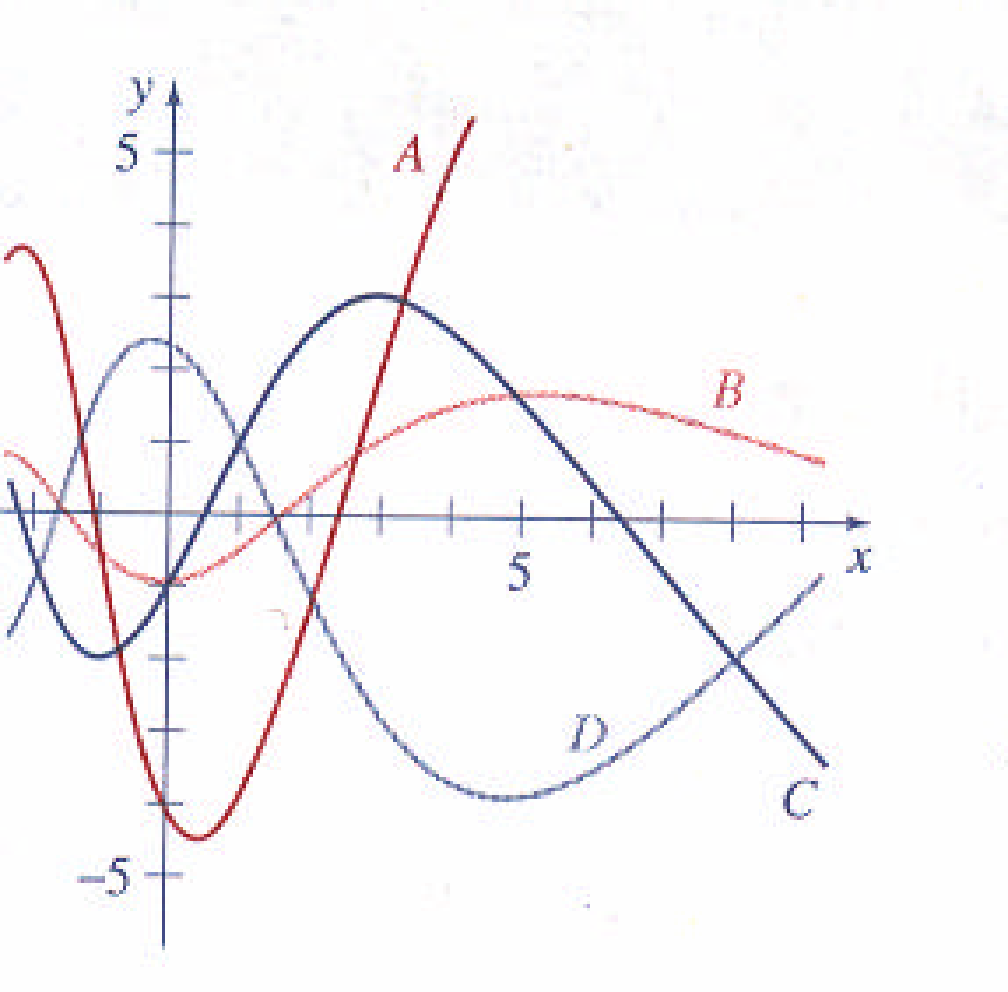
\includegraphics[width= 0.9 \linewidth]{IMAGENES/images/image5.png}
		\end{minipage}
	\item Considere el problema de valores iniciales \(y \,' =x-2y\), \(y(0) = \frac 12\). Determine cuál de las dos curvas que se muestran en la siguiente figura es la única curva solución plausible.\\Explique su razonamiento.
		\begin{figure}[ht]
			\centering
			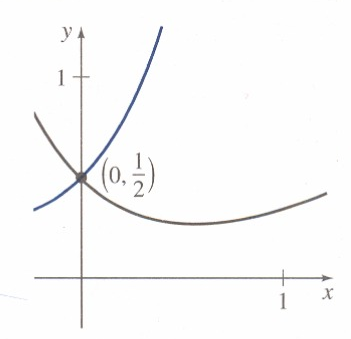
\includegraphics[width= 0.5 \linewidth]{IMAGENES/images/image10.png}
		\end{figure}
\end{enumerate}

\end{document}
